\documentclass{ltjsbook}
\usepackage{docmute} 
\usepackage{../../myStyle} 

\begin{document}
\chapter{数値データの種類}
\label{cb04_Number_and_Data}

さて前回は，科学としての心理学なので，数量的なデータを扱って研究が進められる，という話をしました。今回は，何をどのようにデータにするか，データの種類と言った点についてお話しします。

\section{データと変数}

心理学では目に見えないものを研究対象とするため，心を持つと考えられる主体にたいして刺激を与え，その反応を見て「こうすれば(刺激)$\to$心のせいで$\to$こうなる(反応)」という因果を説明するためのモデルとして研究するのだ，ということでした。ここで刺激と反応は，研究対象である「心」の外にあって，観測できるものです。これをデータにします。

図\ref{fig::03_01}は心理学研究の流れを説明したものです。ここで述べている「刺激と反応からデータを作る」というところは\keytermL{心理測定法}{しんりそくていほう}と呼ばれます。何をどのようにデータにするか，ということを考えるところであり，それぞれの心理学領域によってさまざまなバリエーションがあります。神経生理のような領域での研究であれば，データは計測機から得られる電気反応の強さ，間隔などになるでしょうし，認知・知覚・学習心理学のような領域であれば，たとえば被験者のキー反応の早さなどをPCで計測してデータとするでしょう。社会・学習・臨床心理学のような応用的領域であれば，被験者の発話，調査票への回答パターンなどがデータになるでしょう。いずれの領域でデータを取るにしても，ここで重要なのはそのデータの\keyterm{信頼性}{しんらいせい}{reliability}と\keyterm{妥当性}{だとうせい}{validity}です\footnote{詳しくは第\ref{m06_ctt}講で触れます。}。

\begin{figure}[ht]
	\centering
	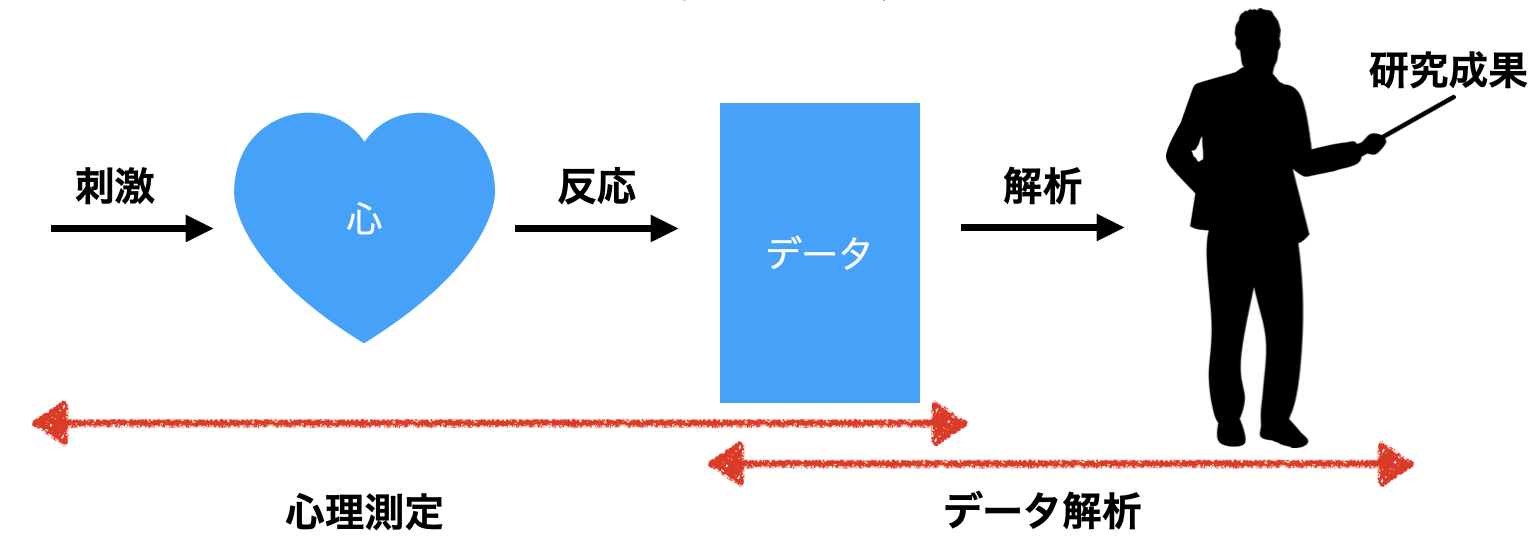
\includegraphics[keepaspectratio,width=0.8\linewidth]{figures/02_Numbers/slide03_01.png}
	\caption{心理学研究のプロセス}
	\label{fig::03_01}
\end{figure}

それに対して，この講義でとくに重点的に議論するのは後半のデータ解析のところになります。つまりデータが得られた後で，それをどのように分析していくか，という点です。これについては次回も言及しますが\footnote{$\to$セクション\ref{reproducibility},Pp.\pageref{reproducibility}}，\keyterm{客観性}{きゃっかんせい}{objectivity}や\keyterm{再現性}{さいげんせい}{reproducibility}が重要になってきます。同じデータであれば誰でも同じ結果に到達できる，ということが重要ですし，言い方を変えると数学的に正誤の判断がついてしまう領域でもありますので，正しく理解し利用できるように学んでいきましょう。

\begin{figure}[ht]
	\centering
	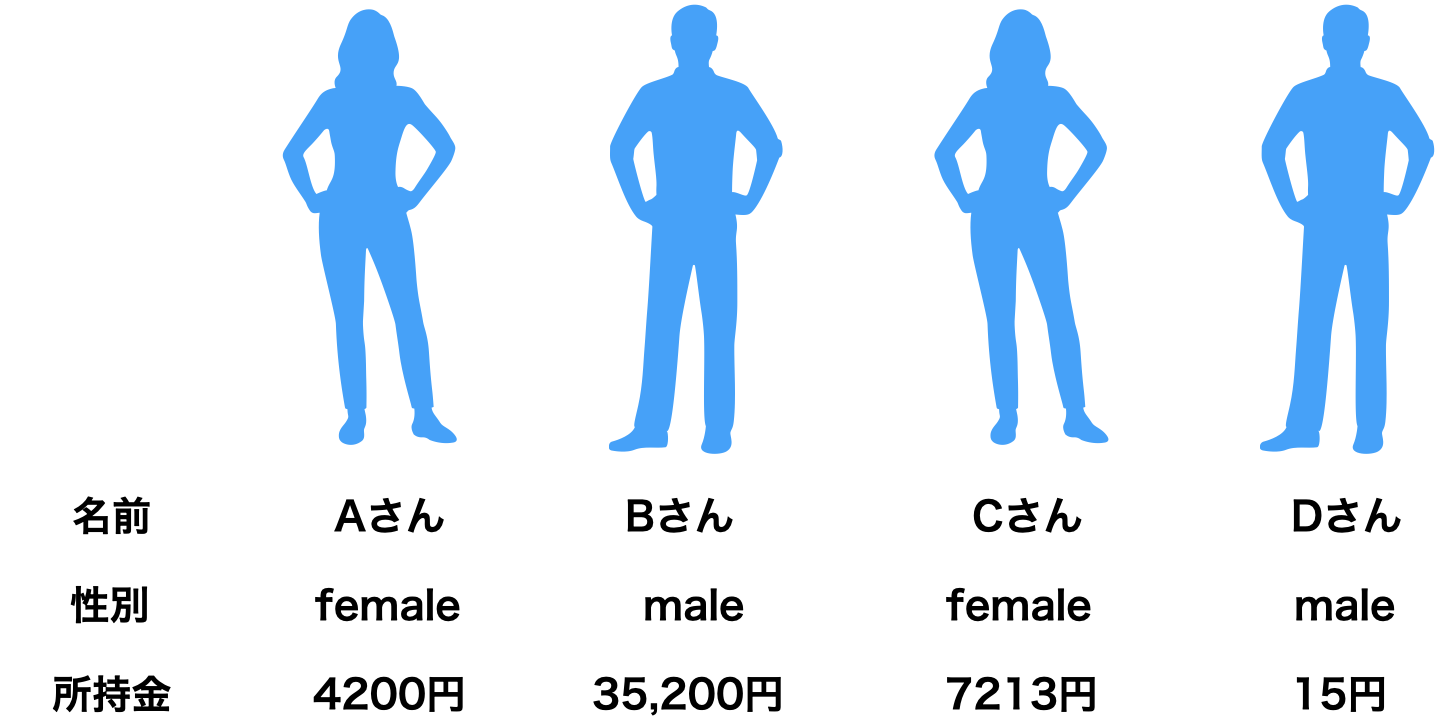
\includegraphics[keepaspectratio,width=0.8\linewidth]{figures/02_Numbers/slide03_02.png}
	\caption{データって何?}
	\label{fig::03_02}
\end{figure}

さてこれからデータを分析していく話をするのですが，改めてデータとは何でしょうか。図\ref{fig::03_02}を見てください。ここには4人の研究対象者がいて，色々な情報を集めてみました。この中でデータとはいったい何を表すでしょうか。所持金は数字ですので，これだけがデータだ，と思ったら大間違いです。実は名前や性別もデータです。これらはすべて数値化し，データとして扱えるものです。

少し用語の説明をしておきますと，名前，性別，所持金などは人によって\footnote{心理学でも研究対象が人でない場合がありますから，データの単位は他にも「個体」「ケース」などということがあります。英語のObservationを略してObs.と書かれることもあります。}変わる数字です。人によって変わる数字のことを\keyterm{変数}{へんすう}{variables}と言います。名前・性別・所持金は変数名であり，それがケースごとに「Aさん」「男性male」「15円」と変わるのです。ここで15円はともかく，名前や性別は数字じゃないぞ？ と思われるかもしれません。先にも述べたように，数字じゃないような実体であっても，これに数字を割り振るルールを決めて数字に置き換えていきます。このルールを決めることを\keyterm{尺度化}{しゃくどか}{scaling}と言います。

\begin{figure}[ht]
	\centering
	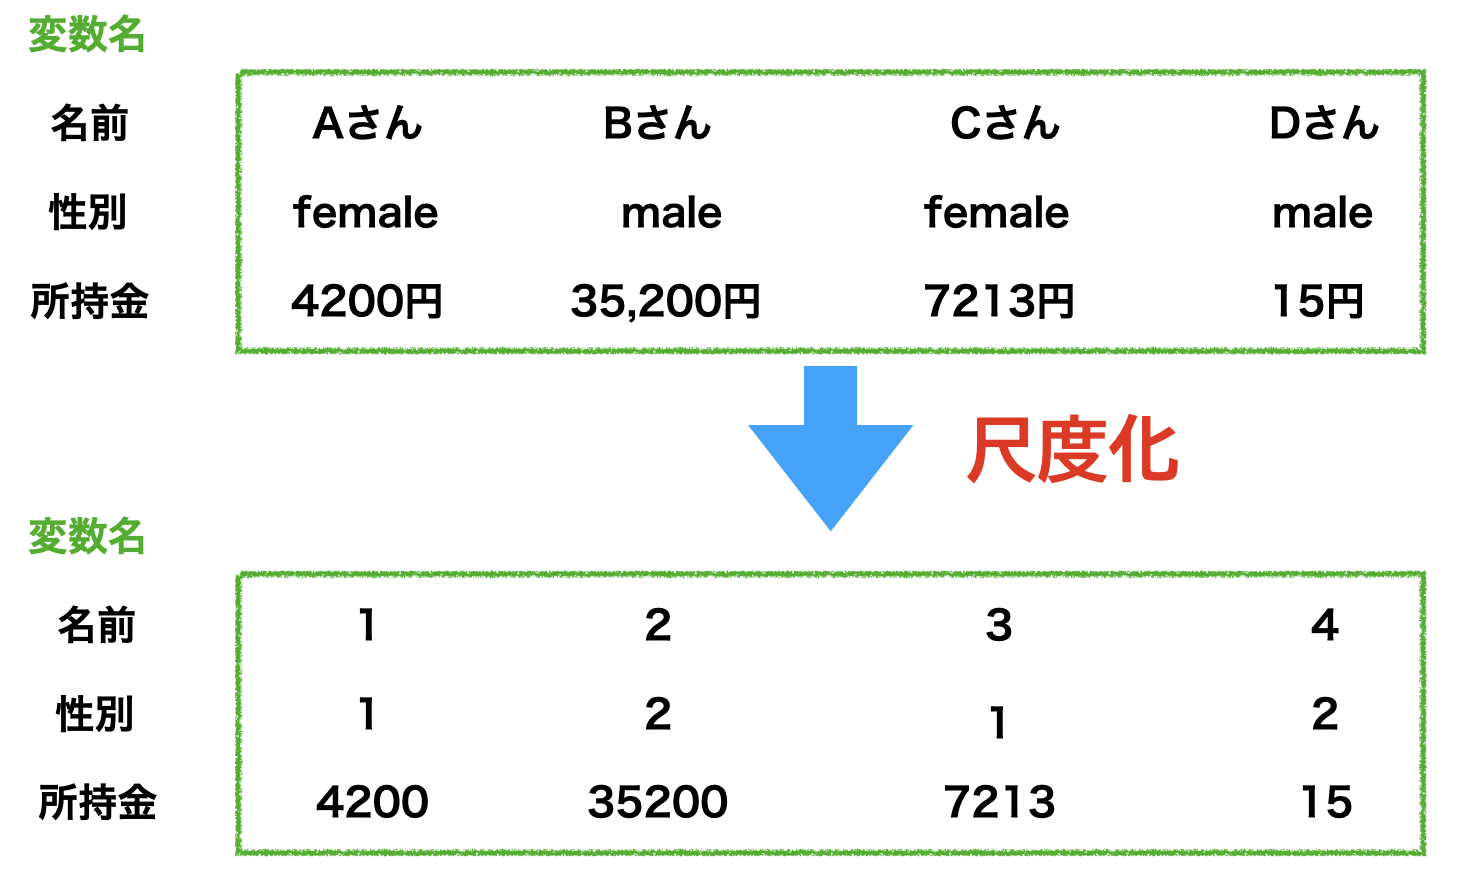
\includegraphics[keepaspectratio,width=0.8\linewidth]{figures/02_Numbers/slide03_03.png}
	\caption{尺度化＝数値に置き換える}
	\label{fig::03_03}
\end{figure}

図\ref{fig::03_03}に数値化した例を挙げました。上の段にあるのが本来の情報であり，数値化されたのが下の段にあります。下の段はすべて数字になっていますね。どこがどう変わっているのか，よく見ておきましょう。実際の統計的な分析をするときは電子計算機を使いますが，電子計算機にデータを与えるときは下の段にあるように数字だけにするのだ，と理解してください\footnote{ExcelやNumbersなどの表計算ソフトでは，その枠の中に日本語を書き込むことができます。しかし統計ソフトで扱う場合は，機械が内部では下段のような数字に置き換えているのだと思っておいてください。電子計算機の中では日本語も0/1の数列にすぎませんが。}。

こうしてみていても，数字には2種類あることがわかります。まず所持金を見てください。これは最初から数字でしたので，そのまま数字として扱っていきます\footnote{単位の「円」という文字は取れています。表計算ソフトに入力するときはこのように，数字以外のものは削ぎ落とすようにしてください。文字が入っていると数字として計算できないからです。ましてや2バイト文字なんて!}。このように本来の数字としての意味を持っているものは\keyterm{量的変数}{りょうてきへんすう}{numeric variable}と呼ばれます。一方で，性別は「女性female」を1に，「男性male」を2に置き換えています。名前に至っては，「Aさん」を1に，「Bさん」を2に，「Cさん」を3に，「Dさん」を4に置き換えています。これらの数字は人や性質を分類するためのものであって，数字に大小関係など量的な違いを表すものではありません。いわば質的な違いを表すための数字で，こうした変数は\keyterm{質的変数}{しつてきへんすう}{categorical variable}と呼ばれます。

このことからわかるように，「なんでも数字にして扱うが，数字には種類がある」ということに注意が必要です。なんでも数字にする，というと眉をひそめる人がいるかもしれません。心・気持ち・想いは数字にできない！と直観的に反論したくなる人もいるでしょう。しかしまったくできないわけではないのです。というのも，言葉にできるのであればそれに適当な数字を割り振ることは可能だからです。数字が必ずしも大小関係を表すものばかりではないこともあるのですから。言葉にできるということは，質的に異なって分類できるということであり，それに数字のラベルを貼ることは可能です。一方，言葉にできない気持ちというのもあるでしょう。しかし，適切に言葉にできないのであれば，科学的な研究対象にはならないと言わざるを得ません。なぜなら「私だけが知りうる本当の気持ち」というのは，私秘性を徹底的に排除するという科学の基本姿勢に反するからです\footnote{言葉に言えないなんとも表現できない気持ちがない，と言ってるわけではないのです。科学的に研究できない，というだけで，私個人も色々な心の動きを経験しています。ただそれは私一人の思い出であって，研究対象にならないと言っているだけです。}\footnote{言葉にして数値化するというのは，心の一側面を捉えているにすぎない，という指摘も当然ありましょう。しかしだからと言って数字を使わない，というのはもったいないのです。また数字で表すことによって，どこまで表現できてどこまで表現できないか，というのも表現できたりします(正確には誤差の大きさを見積もる，という話で本講義の第\ref{m06_ctt}講ごろから触れていきます)。表現できるところはし尽くし，できないところについては黙って味わえば良いのであって，表現することを禁じるのは建設的な態度ではありません。}。

心理学の研究法の1つに，質問紙法というものがあります。複数の項目が並んでいて，それぞれに対して「当てはまる」「どちらかと言えば当てはまる」「どちらとも言えない」「どちらかと言えば当てはまらない」「まったく当てはまらない」のどこかに丸をつけてください，という聞き方をするものが一般的です。たとえば「Q.この世の中では，努力がいつか報われるようになっていると思う」という問いに対して「自分の考え(気持ち，意見，態度)に最も近いところに丸をしてください」と言われ，ある人は「当てはまる」に丸を，別の人は「どちらかと言えば当てはまらない」に丸をつけたとしましょう。ここで「当てはまる」を5点，「どちらかと言えば当てはまらない」を3点，といった形で数値化すれば，大小関係は比較できるので量的変数として扱うことができます。この時ここで測りたいのは，「世界は公平だと思うか」というその人の心理的態度(信念)を測定していると考えられます。

このように回答のパターンを見ることで，目に見えない心の状態を数値化することもできます。見たいものは目に見えない心の状態ですが，測定して，点数をつけたりします。他にも，行動や振る舞いの記録など，知りたいことについて集められる情報はすべてデータであり，分析対象になります。注意してほしいのは，抽象的で目に見えないものだからなんでも好き勝手に「◯◯力」と名付ければいいというものではない，というところです。心理学者は空想世界に住んでいるわけではありません。現実の世界に起こる見て触れることのできるものがあり，それに基づく現象(phenomenon)があります。この現象は抽象的なもので直接その対象が見えるわけではありませんが，現象として観測される何かがあるわけです。たとえば「流行現象」というのはモノやサービスが多くの人に利用される現象ですが，見えるのはそのモノやサービスの利用者でしかありません。ただしそれが多く観測されて，この状態を「流行」と呼ぼう，というわけです。このように抽象化されたものを\keyterm{構成概念}{こうせいがいねん}{theoretical construct}と言います。構成概念は現実や現象に立脚したものですが，構成概念に立脚した別の構成概念というのも考えられます。これは概念同士の関係から論理的に導出されるもので，その概念を設定する意義(その概念がないと説明できない，あるいはその概念があることで他の概念や理論との共通点が見られるなど)がなければなりません。

\begin{figure}[ht]
	\centering
	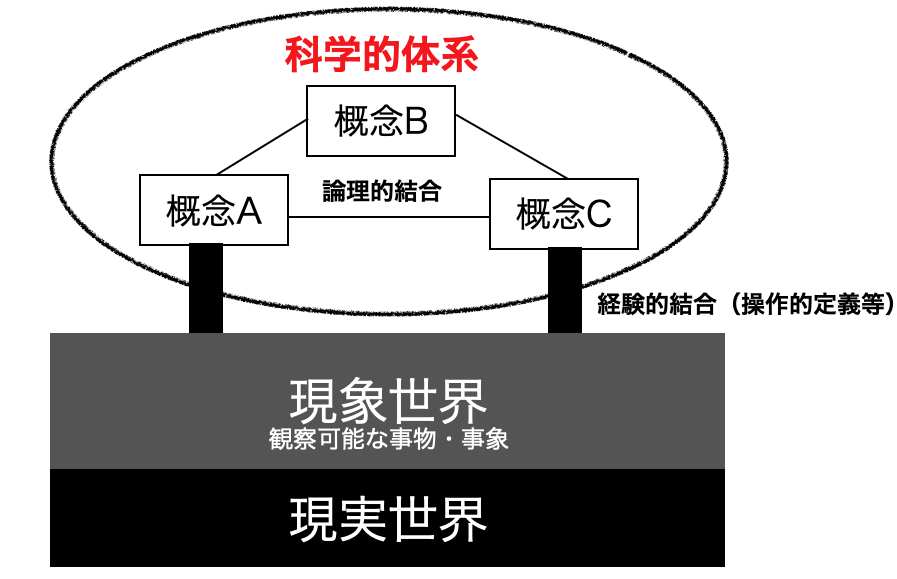
\includegraphics[keepaspectratio,width=0.7\linewidth]{figures/02_Numbers/constructs.png}
	\caption{構成概念と現実との対応(\textcite{Suenaga1987}を元に作図)}
	\label{fig::03_const}
\end{figure}

図\ref{fig::03_const}にあるように，概念は現実や現象に深く根ざした(経験的結合をした)ものであるか，概念同士の関係に強く結び付けられた論理的結合をしたものである必要があります。この抽象的で目に見えないものに対して，筋の通った論理的な説明体系を私たちは科学と呼ぶのです。

\underline{概念を操作して記録・数値化したものが変数となる}，とも言えるでしょう。心理学的な研究対象について，何をどう変数化するか，その結びつきをどう考えるかを知るためには，先行研究を広く調べたり現実世界・現象世界についての知識と教養が必要なのはいうまでもありません。

\section{計算機と統計の観点による分類}
\label{computer_data_type}
さて，心理学ではこのように目に見えて測れるものだけでなく，目に見えないものも数値化して扱います。そしてその数値を計算機に入れて，統計的な処理をしていくことになります。

ここで，計算機の中でそれらがどのように扱われるかを考えてみましょう。統計ソフトRでは，値\footnote{ここでの「値」とは厳密には\keyterm{リテラル}{りてらる}{literal}といい，値の直接的表現のことを指します。}は3つの種類を持ちます。
\begin{itemize}
    \item 数値。言葉の通り数字を数字として扱うということですが，細かく言えば整数，実数，複素数です。また，数学的には無限に続く数列も数字ですが，計算機で無限は表現できないので，必ずどこかに限界があります。数学的な計算と計算機の計算結果が，この限界のせいで少しズレることもあります。また，桁の大きな数字については科学的表記法として，$2e3=2 \times 10^3 = 2000$のような書き方をすることがあります。
    \item 文字列。シングルクォーテーション，あるいはダブルクォーテーションで渡されたものは文字列として扱います。
    \item 論理値。TRUE(真)やFALSE(偽)というのがそれで，TやFの一文字で表現することもあります。条件が成立したかどうか，オプションを使うかどうか，スイッチのオン・オフのような表現をしたい時に使われます。
\end{itemize}
実際に値を付与する時に，どの種類で渡されているかに注意しましょう。たとえば$1$は数値としてあつかわれますが，１(全角文字)は文字として扱われます。計算機上は，半角数字のみが数値として扱われます。

さて，統計分析を進める上では数値にのみ注目することになりますが，統計的な観点から数値変数の種類を次のように分類することができます。この分類は，後に説明する\keyterm{確率変数}{かくりつへんすう}{random variables}との対応を視野にしたものであることを頭の片隅に置いておいてください。確率変数やその確率変数が従う\keyterm{確率分布}{かくりつぶんぷ}{random distribution}については先の話題ではありますが，参考までにここで各変数の対応する確率分布についても記載しておきます。

\paragraph{バイナリ}
\keyterm{バイナリ}{ばいなり}{binary}変数とは，0と1という，2つの値しか持たない変数です。値が二つしかありませんが，それが男と女，生と死，有ると無い，正答と誤答，成功と失敗，オンとオフのように，二分法的な意味を表していると考えると，様々な使い方ができます。もっとも単純だからこそ最もよく使われますし，使い勝手の良い変数でもあります。対応する確率分布としては，\keyterm{ベルヌーイ分布}{べるぬーいぶんぷ}{Bernoulli distribution}というものになります。
\paragraph{カウント}
\keyterm{カウント}{かうんと}{count}変数とは，正の整数しかとらない値のことを指します。年齢，友達の数，来店回数など，数を数える変数です。大きな桁数になれば一度の意味が薄らいできますが，小さな桁数の時は大きな意味がありますね(ex.友達の数が0から1に，1から2に増えることは大きなインパクトがありますが，1000人が1001人になる時はそれほど感動がないかもしれません)。カウント変数は\keyterm{ポアソン分布}{ぽあそんぶんぷ}{Poisson distribution}に従います。
\paragraph{カテゴリ}
\keyterm{カテゴリ}{かてごり}{category}変数とは数値が対象と一対一対応しているもののことを指します。先ほどバイナリ変数は0と1と生と死のように解釈する，と言いましたが，これが3つ以上の種類にあるようなものです。たとえば47都道府県に数字を割り振って，北海道が1で，東京都は13，神奈川県は14...とつけていくことができます。数字と対象の対応であり，この数字を使って計算することはできません。日記や逐語録(インタビューデータ)，SNSでの書き込みなど自然言語を統計解析するときは，単語や文字に数字を割り振って，カテゴリ変数として分析します。カテゴリ変数が従う確率分布は\keyterm{カテゴリカル分布}{かてごりかるぶんぷ}{Categorical distribution}といいます。
\paragraph{連続}
上記以外の変数は基本的に\keyterm{連続}{れんぞく}{continuous}変数である，といいます。数学的に連続であることの定義は難しいですが，ここでは単に「数字と数字の間に別の数字があるようなもの」のことを言う，と理解してください。たとえば身長のことを考えてみます。170cmと175cmの間には172.5cmがあります。170cmと172.5cmの間には，171.25cmがあります。170cmと171.25cmの間には170.625cmがあります。170cmと170.625cmの間には・・・とどこまでも続けていくことが(原理的には)可能ですね。このような数値は連続しているといい，確率分布はさまざまなものが対応します。代表的には\keyterm{正規分布}{せいきぶんぷ}{Normal distribution}などがあります。ちなみに，連続でない変数(バイナリ，カウント，カテゴリ)は，\keyterm{離散的}{りさんてき}{discrete}変数，と言います。

ここで知っておいてほしいことは，文字や文といった文字型のデータであっても数字を割り振って統計的に分析することができる，ということです。計算機で分析する以上，内部的にも概念的にも，全て数字を割り当てて考えるのだということを知っておいてください。

進んだ統計モデルを扱うときは，対応する確率分布に応じて使う手法が変わってきたりします。それほど発展的な分析でないとしても，データにどのような計算が許されるかについては考えておかなければなりません。この「データにどのような計算が許されるか」については\keytermL{尺度水準}{しゃくどすいじゅん}を知らなければなりません。

\section{尺度水準による分類}
変数にはさまざまな名称があることを見てきました。尺度化して数字になってしまえば全部同じか，というと実はそうではありません。\textcite{stevens1946}は数値が持つ情報とそれに伴う計算可能性の観点から，尺度を4つの水準に分類しています。それぞれ次のような名前がついています。
\begin{enumerate}
	\item \keyterm{名義尺度水準}{めいぎしゃくどすいじゅん}{nominal scale}
	\item \keyterm{順序尺度水準}{じゅんじょしゃくどすいじゅん}{ordinal scale}
	\item \keyterm{間隔尺度水準}{かんかくしゃくどすいじゅん}{interval scale}
	\item \keyterm{比率尺度水準}{ひりつしゃくどすいじゅん}{ratio scale}
\end{enumerate}

名義尺度水準が最も下のレベルで，比率尺度水準が最も上のレベルという階層性を持っています。上に上がるほど徐々に条件が強くなっていきます。逆に言えば，上の尺度水準に該当する変数をより下位の水準の変数として扱うことが可能です。このことについて詳しくは後ほど説明するとして，それぞれがどういう意味なのかを説明していきましょう。

\paragraph{名義尺度水準}
最も下位のレベルにある水準です。この水準にある数値は，数字ではありますが数字としての意味がないレベルです。単にラベルとして対象に数字を割り当てた，というだけのとき，その数字は\keytermL{名義尺度水準}{めいぎしゃくどすいじゅん}にある，と言います。この講のセクション\ref{chap3sec2},Pp.\pageref{chap3sec2}で，性別や名前に数字を割り当てたのを思い出してください。たとえば女性に1を，男性に2を割り当てたとします。この割り当てられた数字に，深い意味はないですね。別に男性が2でもいいし，女性に43543という数字を当てておいても良いわけです。数字だけ見ても，女性が男性の2倍あるとか，男性より少ない・小さいことを意味しているわけではありません。あるいはみなさんが持っている携帯電話の番号もこの尺度水準です。みなさんの数字はどれひとつとして同じではないですが，その数字に深い意味はないですね\footnote{語呂合わせがしやすいかどうか，というのはありますが。}。他にも学籍番号や，名前に割り当てられた数字(Aさんが1,Bさんが2など)に数字としての特徴はなく，ただの名前を簡略化したものに過ぎません。こういう数字のことを名義尺度水準にある数字，というわけです。

この水準の数字は，数字が大小関係や順序関係を表さないので，計算ができません。たとえば女性を1，男性を2と尺度化したデータを集めて平均値を出したら1.7でした，と言っても意味がないのです。1.7に該当する対象がないのですから。この尺度水準では\texttt{数字と対象が一対一対応していること}が重要なのであって，数字を計算して変化させても意味がありません。ではこの尺度水準の数字はなんの役にも立たないのか，と言われるとそんなことはありません。違う数字が割り振られていることから違う対象であることは分かりますので，分類するという性質は持っていますし，何よりどんな複雑な対象であっても名義尺度水準の数値は割り当てられるのです。その意味では，この後に出てくるどんな尺度水準よりも豊富な情報を含んでいる数値である，とも言えます。また，言葉にできなければ研究対象にできないという話をしましたが，言い換えると言葉にできるのであれば名義尺度水準の数値が割り当てられるということでもあります。

\paragraph{順序尺度水準}
名義尺度水準は数字としての意味を持たない，と言いました。これに順序関係，すなわち数字の大小に意味があるという条件が加われば，それは\keytermL{順序尺度水準}{じゅんじょしゃくどすいじゅん}の数字だということができます。たとえば好きな夕飯のメニューとして1番がカレー，2番がハンバーグだと答えた人がいたら，カレーの方がハンバーグよりも好まれている，価値が高い，優先されているという情報は得られるわけです。あるいは100m走での順位を表す数字だと，2と7を比べれば2位の人の方が速いんだな，ということがわかります。この程度の情報が含まれている数字のことを，順序尺度水準であると言います。ただこの水準の数字は大小関係を表すだけで，それ以外のことはわかりません。たとえば着順の話でも，1，2，3の順で優劣がついていることはわかるのですが，「1位がぶっちぎりだった」「団子レースだった」といった違いは表現できていないわけです。図\ref{fig::03_05}を見てもらうとわかるように，データとしては1,2,3という数字だけですから，上図のような状態でも下図のような状態でもデータとしては1,2,3,4であり，上図の2と下図の2を区別できません。まだ少し不便ですね。このように大小しかわからないので，計算にもまだ使えません。1位と2位を足して3位になるはずもないですし(そもそも逆転してますが)，2位と3位を足して1位と勝負できるかということもわからないのです。もちろんかけたり割ったりもできませんので，この水準の数字は四則演算ができません。

\begin{figure}[ht]
	\centering
	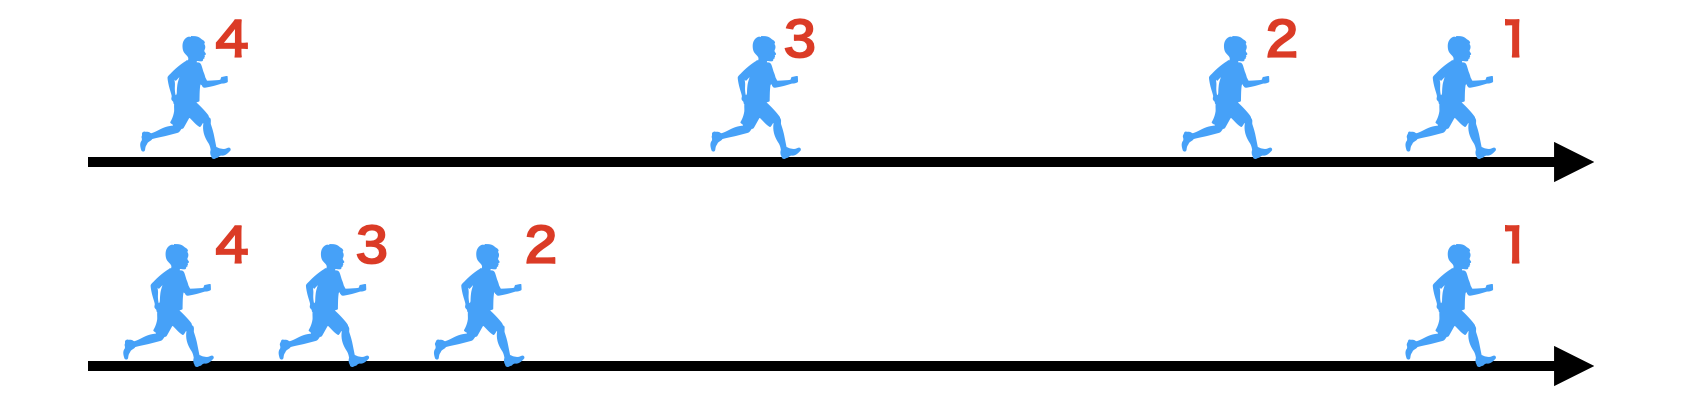
\includegraphics[keepaspectratio,width=0.8\linewidth]{figures/02_Numbers/slide03_05.png}
	\caption{順序では程度がわからない}
	\label{fig::03_05}
\end{figure}

とはいえ，この水準の数字は，心理測定において最もおもしろいところであると言えるかもしれません。みなさんご自身の心の状態を数字で表すとして，さてその数字はどの水準にあるのでしょうか。たとえば「カレーはハンバーグの100倍美味しい！」と思っていても，本当に100倍という計算ができるような精度の高い数字でしょうか？ せいぜい優先順位の違いぐらいで，カレーを5点，ハンバーグを4点，餃子を3点・・・と採点していっても，カレーとハンバーグの違いが，ハンバーグと餃子との差と同程度であるとまでは言えないのではないでしょうか。ことほど左様に，心理学的な評価水準はせいぜい順序尺度水準であって，差や比の計算をするには，さらに上の尺度水準でなければなりません\footnote{しかし実際には，評定値を間隔尺度水準の値を持っているとみなして分析をすることが多くあります。これには\keytermL{心理測定法}{しんりそくていほう}の理論と歴史的な経緯があって，その両方を踏まえた上でことであればそのような「みなし」も正当化されます。残念なことに，それらを踏まえずして仮定が満たされていないのに勝手に間隔尺度水準だと思って使っている誤用例も数多くあるのですが。}。

\paragraph{間隔尺度水準}
\keytermL{間隔尺度水準}{かんかくしゃくどすいじゅん}は，順序尺度水準に加えて数値と数値の間隔が等しいという条件を追加したものです。順序尺度水準は1と2の差が2と3の差と違っても構わないのですが，間隔尺度水準ではこれがあっている必要があります。
代表的な例として，摂氏(温度)があげられます。これは水が氷になる氷点を0，水が水蒸気になる沸点を100とし，その間隔を百等分した目盛りによって温度を表現するものです\footnote{セルシウスさんが考えた方法なのでセ氏といいます。ちなみに定義上このようになっているのであって，「水ってちょうど0度で氷になって，ちょうど100度で水蒸気になるの，奇跡じゃない?」というのは悪いジョークです。}。このようにそもそも等間隔になるようにつけた目盛りですから，当然間隔尺度水準の数値であると言えます。この時，10℃と20℃の差は20℃と30℃の差と等しいといえますから，これは$20-10=30-20$と引き算の計算ができるレベルになっているわけです。

しかし，10℃は20℃の2倍の熱量を持っている，とは言えません。というのも，この数字は0℃に意味がないからです。言い換えると，0℃は温度が「ない」ことを意味するのではなく，0℃という温度が「ある」状態です。0がスタート地点ではないのです。スタート地点は任意に決められますから，たとえば
氷点を100，沸点を200とした新しい温度体系Xを作ったとします。このとき10℃は110Xで，20℃は120Xですから，$20/10\neq 120/110$ですね。同じ状態を表している数字なのに計算が合わないのはおかしいわけです。このような割り算の計算をするためには，さらにもうひとつ条件を追加する必要があります。

\paragraph{比率尺度水準}
\keytermL{比率尺度水準}{ひりつしゃくどすいじゅん}は，間隔尺度水準に加えて絶対0点を定めたものです。絶対0点とは，0が「ない」ことを意味する点のことです。たとえば0cmは長さがないのです。0kgは重さがないし，0秒は時間が経ってない，です。このように原点0が決まっている数値体系になってはじめて，加減乗除の四則演算すべてに対応できます。例に挙げたように，物理的な測定単位はほとんど比率尺度水準ですから，精緻に測定すればかなり細かい予測値まで計算できるのですね。これに対して心理学のデータで主観的につけられる評定値はせいぜいが順序尺度水準なので，物理学のようになかなかうまくいかないところもあるというのが実際です。心理学のデータでも客観的で比率尺度水準の数字を扱えるものもありますし(反応時間を指標とする，など)，主観的な評定値でも工夫して間隔尺度水準以上の数値にすることもあります。

みなさんが今後，どのようなデータをとって分析するようになるかは進む専門領域によって変わると思いますが，どの数字がどの尺度水準にあるのかについて，常に注意しておいてください。というのも，名義尺度水準や順序尺度水準では加減乗除の計算ができないので，分析の方法にも限界があるからです。これら尺度水準の違いは，統計ソフトウェアで分析するときもどの尺度水準にあるのか指定する必要があります。指定がなくすべて計算可能な数値であると機械が誤認すると，頓珍漢な分析をしてしまうことになります。表\ref{tab::03_01}に\textcite{stevens1946}によるまとめを引用しましたので確認しておいてください\footnote{\textcite{stevens1946}の仕事をより正確に言うなら「測定対象全体に数値を与える適正な規則とは何か」を考えたのではなく，何らかの測定がなされた尺度がいくつかあれば，それらを相互に変換する規則が定められて，それが表にあるような4種類になるだろう，と言う考え方です。詳しくは\textcite{Yoshino2007}を参照してください。}。

\begin{table}[ht]
	\centering
	\caption{尺度水準のまとめ}
	\begin{tabular}{cccc}
		尺度水準                                         & 基本的な操作       & 数学的な群構造                                                           & 可能な統計量                                                      \\\hline
		\begin{tabular}{c}名義\\Nominal\end{tabular}   & 同質性の判定       & \begin{tabular}{c} 置換群 \\ $x'=f(x)$\\$f(x)$は一対一対応  \end{tabular}  & \begin{tabular}{c}ケース数,\\最頻値,\\一致係数\end{tabular}            \\\hline
		\begin{tabular}{c}順序\\ Ordinal\end{tabular}  & 大小関係の判定      & \begin{tabular}{c} 同調群 \\  $x'=f(x)$\\$f(x)$は単調増加関数 \end{tabular} & \begin{tabular}{c}中央値, \\パーセンタイル\end{tabular}               \\\hline
		\begin{tabular}{c}間隔\\ Interval\end{tabular} & 間隔や差分の等しさの判定 & \begin{tabular}{c} 一般線形群\\$x' = ax + b$ \end{tabular}             & \begin{tabular}{c}平均値 ,\\ 標準偏差,\\  順序相関,\\積率相関\end{tabular} \\\hline
		\begin{tabular}{c}比率\\ Ratio\end{tabular}    & 比率の等しさの判定    & \begin{tabular}{c} 類似性群\\$x'=ax$ \end{tabular}                    & \begin{tabular}{c}変動係数 \end{tabular}                        \\\hline
	\end{tabular}
	\label{tab::03_01}
\end{table}

\section{コンピュータのデータ型と尺度水準の関係}
ここまで，計算機による値の分類と，尺度同士の変換関係すなわち値に施せる計算の関係から変数を分類してきました。では，計算機のデータと尺度水準との関係はどのようになっているでしょうか。

最も単純には，間隔尺度水準と比率尺度水準はいずれも計算できるので量的データ，名義尺度水準と順序尺度水準は(計算できないので)質的なデータと呼ぶことがあります。しかし，カウントデータを順序尺度水準として扱うこともできますし，比率尺度水準であると考えることもできるでしょう。
またバイナリデータは特殊で，2つしか状態がないので名義尺度水準であるとも言えるし，最も単純な段階を持つ順序尺度水準であるとも言えるし，数学上は比率尺度水準であると考えて計算しても良いのです。

また，調査法によって得られた数字，たとえば「非常にそう思う」を5点，「全くそう思わない」を1点とする，といった5段階の点数の付け方は，統計学的には順序尺度水準として扱うことが正しいです。\textbf{しかしながら}実践的には，間隔尺度水準とみなして分析することが多いです。その理由の一つは，かつて計算機の計算能力が今ほど高くなかった時代に，順序尺度水準の統計モデルは理論的に考えられていても，実質的に計算時間がかかりすぎるので使えないから，という歴史的背景があります。もちろん今はそんなことはありませんので，順序尺度水準は順序尺度水準として正しい統計モデルを利用するべきでしょう\footnote{もうひとつ，調査法の多段階反応項目について，各カテゴリにはある仮定のもとで連続量を割り振る方法が考えられており，その手法を使うと理論的に間隔尺度水準の数字として扱えるという研究があります。サーストンの等現間隔法やシッカートのシグマ法と呼ばれるものがそれですが，最近ではこれらの計算における仮定を無視し，単純に1から5までの整数値を割り振る研究が後を立ちません。この辺りの悲喜交々については，別の講義でご紹介する機会があるかと思います。}。

さて，最後に統計ソフトRでは数値や尺度水準をどのように扱えるのかをみてみましょう。
サンプルデータとして\verb|BaseballDecade.csv|というデータセットを使います\footnote{このデータセットはこの資料を提供しているサイト，\url{https://kosugitti.github.io/psychometrics_syllabus/}からダウンロードできます。}。サンプルデータをこの授業のプロジェクトフォルダに保存し，次のコードで読み込んでみましょう。

\begin{lstlisting}[language=c++,label={code:4_01},caption={データの読み込み}]
rm(list = ls())
dat <- read.csv("BaseballDecade.csv",na.strings = "NA")
str(dat)
\end{lstlisting}

\paragraph{コード解説}
\begin{description}
	\item[1行目] 環境の初期化
	\item[2行目] データファイルの読み込み
	\item[3行目] データの構造を見る関数
\end{description}

これを実行すると，次のような出力が得られると思います。
\begin{Rscreen}{外部データの読み込み}{readcsv}
\begin{verbatim}
> str(dat)
'data.frame':	6546 obs. of  17 variables:
 $ Year      : chr  "2011年度" "2011年度" "2011年度" "2011年度" ...
 $ Name      : chr  "永川　勝浩" "前田　健太" "栗原　健太" "東出　輝裕" ...
 $ team      : chr  "Carp" "Carp" "Carp" "Carp" ...
 $ salary    : int  12000 12000 12000 10000 9000 8000 8000 7500 7000 6600 ...
 $ bloodType : chr  "O型" "A型" "O型" "A型" ...
 $ height    : int  188 182 183 171 201 183 177 173 176 188 ...
 $ weight    : int  97 73 95 73 100 90 82 73 80 97 ...
 $ UniformNum: int  20 18 5 2 70 17 31 6 1 43 ...
 $ position  : chr  "投手" "投手" "内野手" "内野手" ...
 $ Games     : int  19 31 144 137 19 6 110 52 52 40 ...
 $ AtBats    : int  NA NA 536 543 NA NA 299 192 44 149 ...
 $ Hit       : int  NA NA 157 151 NA NA 60 41 11 35 ...
 $ HR        : int  NA NA 17 0 NA NA 4 2 0 1 ...
 $ Win       : int  1 10 NA NA 0 1 NA NA NA NA ...
 $ Lose      : int  2 12 NA NA 0 1 NA NA NA NA ...
 $ Save      : int  0 0 NA NA 0 0 NA NA NA NA ...
 $ Hold      : int  0 0 NA NA 9 0 NA NA NA NA ...
\end{verbatim}
\end{Rscreen}
出力から，読み込んだファイルがdata.frame型になっていることがわかります。また，変数がいろいろあり，それぞれの型が示されています。\verb|char|とあるのはcharacter，つまり文字型です。\verb|int|とあるのはinteger，つまり整数である，ということです。数値型は，\verb|int|のほかにも，\verb|num|，つまりnumeric(数字)である，となることもあります。

表示の中で\verb|NA|とあるのは\keyterm{欠測値}{けっそくち}{missing value}です。ある観測(observation)においてその変数の値がなかった時にこのように表示されます。ファイルを読み込む時に，欠測値に対応する文字列を指定しておけばよく，ピリオド(\verb|.|)やアスタリスク(\verb|*|)，特定の値(\verb|-99|など)を仮に入れておいて，分析の時に欠測を表しているものとして指定することが一般的です。

さて，ここで変数\verb|bloodType|をみてみましょう。選手の血液型情報がありますが，これはせいぜいA,B,O,AB型の4つです。すなわちカテゴリ変数であり，文字列としての意味はなく群分けのラベルがついているだけです。尺度水準でいうところの名義尺度水準ですので，そのように扱ってもらうべく変換する必要があります。次のコードを実行してみてください。


\begin{lstlisting}[language=c++,label={code:4_02},caption={Factor型に変換する}]
dat$bloodType <- factor(dat$bloodType)
str(dat$bloodType)
levels(dat$bloodType)
\end{lstlisting}
    
\paragraph{コード解説}
\begin{description}
    \item[1行目] 変数を要因(Factor)型にして上書き保存する
    \item[2行目] 当該変数の構造を確認する
    \item[3行目] 水準を確認する 
\end{description}

実行すると次のように出力されるはずです。
\begin{Rscreen}{因子型の確認}{factor}
\begin{verbatim}
> str(dat$bloodType)
 Factor w/ 5 levels "AB型","A型","B型",..: 4 2 4 2 5 3 2 3 1 5 ....
> levels(dat$bloodType)
[1] "AB型" "A型"  "B型"  "O型"  "不明"
\end{verbatim}
\end{Rscreen}
Rにおける名義尺度水準の変数は要因型(Factor型)と呼ばれます。今回は\verb|factor|関数で変数を要因型に変換しました。出力された結果をみると5つのレベル(水準)がある要因型であることがわかります。続く出力ではAB型に1,A型に2，B型に3，O型に4，不明に5という数字が割り振られていることがわかります。

同様のことは，\verb|team|変数や\verb|position|変数に対してもやっておくと良いでしょう。ただし，文字列変数の全てが要因型(名義尺度水準)であるとしなくても構いません。たとえば\verb|Name|変数(選手の名前)はひとりにひとつ，個別の水準がありますから，水準数が多すぎますので，統計的な処理を必要としないかもしれないからです(水準として設定し，カウントすることに意味があるようなら変換しておきましょう)。

また，\verb|Year|変数は日本語を含みますので文字型になっていますが，扱うなら年度の順番を考慮した順序尺度水準にするべきですね。次のコードを実行してみましょう。

\begin{lstlisting}[language=c++,label={code:4_03},caption={Ord.Factor型に変換する}]
dat$Year <- factor(dat$Year, ordered = TRUE)
str(dat$Year)
levels(dat$Year)
\end{lstlisting}
    
\paragraph{コード解説}
\begin{description}
    \item[1行目] 変数を順序月要因(Ordered Factor)型にして上書き保存する
    \item[2行目] 当該変数の構造を確認する
    \item[3行目] 水準を確認する 
\end{description}

実行すると次のように出力されるはずです。
\begin{Rscreen}{順序つき因子型の確認}{Ord.factor}
\begin{verbatim}
> str(dat$Year)
 Ord.factor w/ 10 levels "2011年度"<"2012年度"<..: 1 1 1 1 1 1 1 1 1 1 ...
> levels(dat$Year)
 [1] "2011年度" "2012年度" "2013年度" "2014年度" "2015年度" "2016年度" "2017年度" 
 [8] "2018年度" "2019年度" "2020年度"
\end{verbatim}
\end{Rscreen}

順序つき要因型はOrdered Factorといいます。これを見ると年度ごとの大小関係が含まれた要因型としてRが受け止めていることがわかります。

Rは要因型に応じて，自動的に適切な統計処理，統計モデルに変えてくれる機能がありますので，データセットを読み込んだらまず，含まれる変数を適切な型に変えておくことは重要です。ちなみに変数の「型」はデータ型とかクラスとか呼ばれます。Rでは主に以下のような分類があります。

\begin{description}
    \item[基本データ型]~
    \begin{description}
        \item[$\bullet$] numeric（数値型：integer、doubleを含む）
        \item[$\bullet$] character（文字列型）
        \item[$\bullet$] logical（論理値型）
        \item[$\bullet$] complex（複素数型）
    \end{description}
    
    \item[特殊データ型]~
    \begin{description}
        \item[$\bullet$] factor（因子型）：カテゴリカルデータ用
        \item[$\bullet$] Date（日付型）
        \item[$\bullet$] POSIXct/POSIXlt（日時型）
        \item[$\bullet$] function（関数型）
    \end{description}
\end{description}

\section{課題}
\paragraph{変数を見つける}次のような研究計画を立てた時に，変数として記録しておくべきなのは何でしょうか。
\begin{enumerate}
	\item 人の身長と体重の情報から，性別を予測することに興味がある。
	\item 人は寝ている間にたくさんの汗をかくという。一晩にかく平均的な寝汗の量に男女差があるのかどうかを調べたい。
	\item 結婚している人としていない人とで，幸福度に差があるかどうかを知りたい。
\end{enumerate}

\paragraph{尺度水準を理解する}次のそれぞれのデータは，どの尺度水準に該当するでしょうか。
\begin{enumerate}
	\item 個人を識別するために回答を求めた携帯電話番号の下4桁の数値
	\item 納税証明書に記載されている，個人の昨年度の納税額
	\item 年齢を直接質問するのがはばかられたため，「10代」「20代」「30代」「40代」「50代以上」の5段階について回答を求め，それぞれ1,2,3,4,5とコード化した数値
	\item 質問に対して「とてもそう思う」を5，「まったくそう思わない」を1として，両者の間を均等に分割し2,3,4とする。また，「答えたくない」を0としてコード化した数値
	\item セルシウスさんが開発した，沸点を100，氷点を0として百分割した温度
	\item 温度とは分子の平均運動量であり，一定量の物質の温度をどんどん下げていくとこれ以上低くはならないという点が出てくる。そこを原点として作られた絶対温度K
	\item テレビ番組「帰れま10」では，ある外食チェーン店の豊富なメニューの中から，上位10品が何であるかを当てなければならない。このとき，それぞれのメニューに付される人気の順位を表した数字
\end{enumerate}

\paragraph{Rでの尺度水準}サンプルデータ\verb|BaseballDecade.csv|を読み込み，因子型にするべき変数は全て因子型にしてみよう。


\end{document}